\section{Experimental Results}
\label{sect:results}

All our experiments were conducted on a 6 core, 3.7 GHz, Intel i7-8700K running an Ubuntu 18.04 operating system. 

\subsection*{{\bf RQ1: How well do planners recommendations match  developer actions?}}
\def\rot{\rotatebox}
\newcolumntype{a}{>{\columncolor{gr1}}r}
\newcolumntype{b}{>{\columncolor{gr2}}r}
\newcolumntype{c}{>{\columncolor{gr3}}r}
\newcolumntype{d}{>{\columncolor{gr4}}r}
\begin{figure}[!htbp]
% \centering
% \arrayrulecolor[gray]{0.5}
% \resizebox{\linewidth}{!}{
% \begin{tabular}{@{}l|rrar|rrrb|rrrc|rrrd}
%             \rowcolor{white}& \multicolumn{4}{c|}{$0\leq Overlap<25$}       & \multicolumn{4}{c|}{$25\leq Overlap<50$}       & \multicolumn{4}{c|}{$50\leq Overlap<75$}       & \multicolumn{4}{c}{$75\leq Overlap\leq100$}      \bigstrut\\ \hline
%             & \rot{90}{ALVES} & \rot{90}{OLIVE} & \rot{90}{SHATW} & \rot{90}{XTREE} & \rot{90}{ALVES} & \rot{90}{OLIVE} & \rot{90}{SHATW} & \rot{90}{XTREE} & \rot{90}{ALVES} & \rot{90}{OLIVE} & \rot{90}{SHATW} & \rot{90}{XTREE} & \rot{90}{ALVES} & \rot{90}{OLIVE} & \rot{90}{SHATW} & \rot{90}{XTREE} \bigstrut\\ \hline
% ant-1      & 139   & 137   & 147   & 14    & 8     & 8     & 4     & 48    & 2     & 2     & 0     & 34    & 3     & 4     & 0     & 76    \bigstrut\\
% ant-2      & 252   & 249   & 263   & 15    & 11    & 10    & 0     & 76    & 1     & 2     & 0     & 45    & 0     & 0     & 0     & 153   \bigstrut\\ 
% ant-3      & 291   & 286   & 312   & 40    & 27    & 25    & 3     & 115   & 3     & 6     & 0     & 71    & 0     & 2     & 0     & 136   \bigstrut\\ \hline
% lucene-1   & 159   & 150   & 182   & 9     & 38    & 29    & 33    & 70    & 24    & 15    & 0     & 38    & 5     & 24    & 0     & 113   \bigstrut\\ \hline
% ivy-1      & \cellcolor{gr1}{39}    & \cellcolor{gr1}{39}    & 39    & 7     & 0     & 1     & 0     & 15    & 0     & 0     & 0     & 8     & 0     & 0     & 0     & 13    \bigstrut\\ \hline
% camel-1    & 437   & 431   & 513   & 119   & 33    & 34    & 0     & 115   & 34    & 16    & 0     & 70    & 23    & 42    & 0     & 248   \bigstrut\\ 
% camel-2    & 720   & 708   & 770   & 44    & 36    & 28    & 0     & 146   & 30    & 16    & 0     & 103   & 2     & 25    & 0     & 527   \bigstrut\\ \hline
% xerces-1   & 363   & 361   & 390   & 4     & 8     & 6     & 0     & 23    & 12    & 6     & 0     & 34    & 14    & 19    & 0     & 343   \bigstrut\\
% xerces-2   & 281   & 278   & 296   & 4     & 7     & 6     & 0     & 17    & 8     & 5     & 0     & 18    & 2     & 10    & 0     & 268   \bigstrut\\ \hline
% velocity-1 & 138   & 127   & 187   & 12    & 32    & 15    & 23    & 29    & 23    & 18    & 0     & 44    & 7     & 34    & 0     & 119   \bigstrut\\ \hline
% xalan-1    & 526   & 517   & 552   & 8     & 45    & 31    & 133   & 94    & 89    & 32    & 85    & 104   & 71    & 123   & 0     & 523   \bigstrut\\
% xalan-2    & 607   & 591   & 773   & 69    & 93    & 24    & 0     & 64    & 114   & 90    & 0     & 198   & 7     & 87    & 0     & 500   \bigstrut\\ \hline
% poi-1      & 268   & 265   & 271   & 3     & 3     & 2     & 13    & 7     & 11    & 2     & 0     & 8     & 1     & 13    & 0     & 265   \bigstrut\\
% poi-2      & 291   & 231   & 323   & 9     & 77    & 81    & 24    & 159   & 20    & 20    & 0     & 50    & 0     & 22    & 0     & 153   \bigstrut\\ \hline
% log4j-1    & 84    & 80    & 92    & 2     & 6     & 8     & 2     & 22    & 5     & 2     & 0     & 16    & 0     & 4     & 0     & 56    \bigstrut\\ \hline
% jedit-1    & 244   & 236   & 249   & 12    & 13    & 13    & 14    & 58    & 8     & 8     & 0     & 57    & 0     & 5     & 0     & 153   \bigstrut\\
% jedit-3    & 194   & 189   & 198   & 31    & 6     & 12    & 1     & 86    & 2     & 2     & 0     & 38    & 0     & 1     & 0     & 77    \bigstrut\\
% jedit-2    & 245   & 238   & 259   & 26    & 16    & 22    & 3     & 102   & 4     & 3     & 0     & 48    & 0     & 3     & 0     & 119   \bigstrut\\ 
% \end{tabular}}
\centering
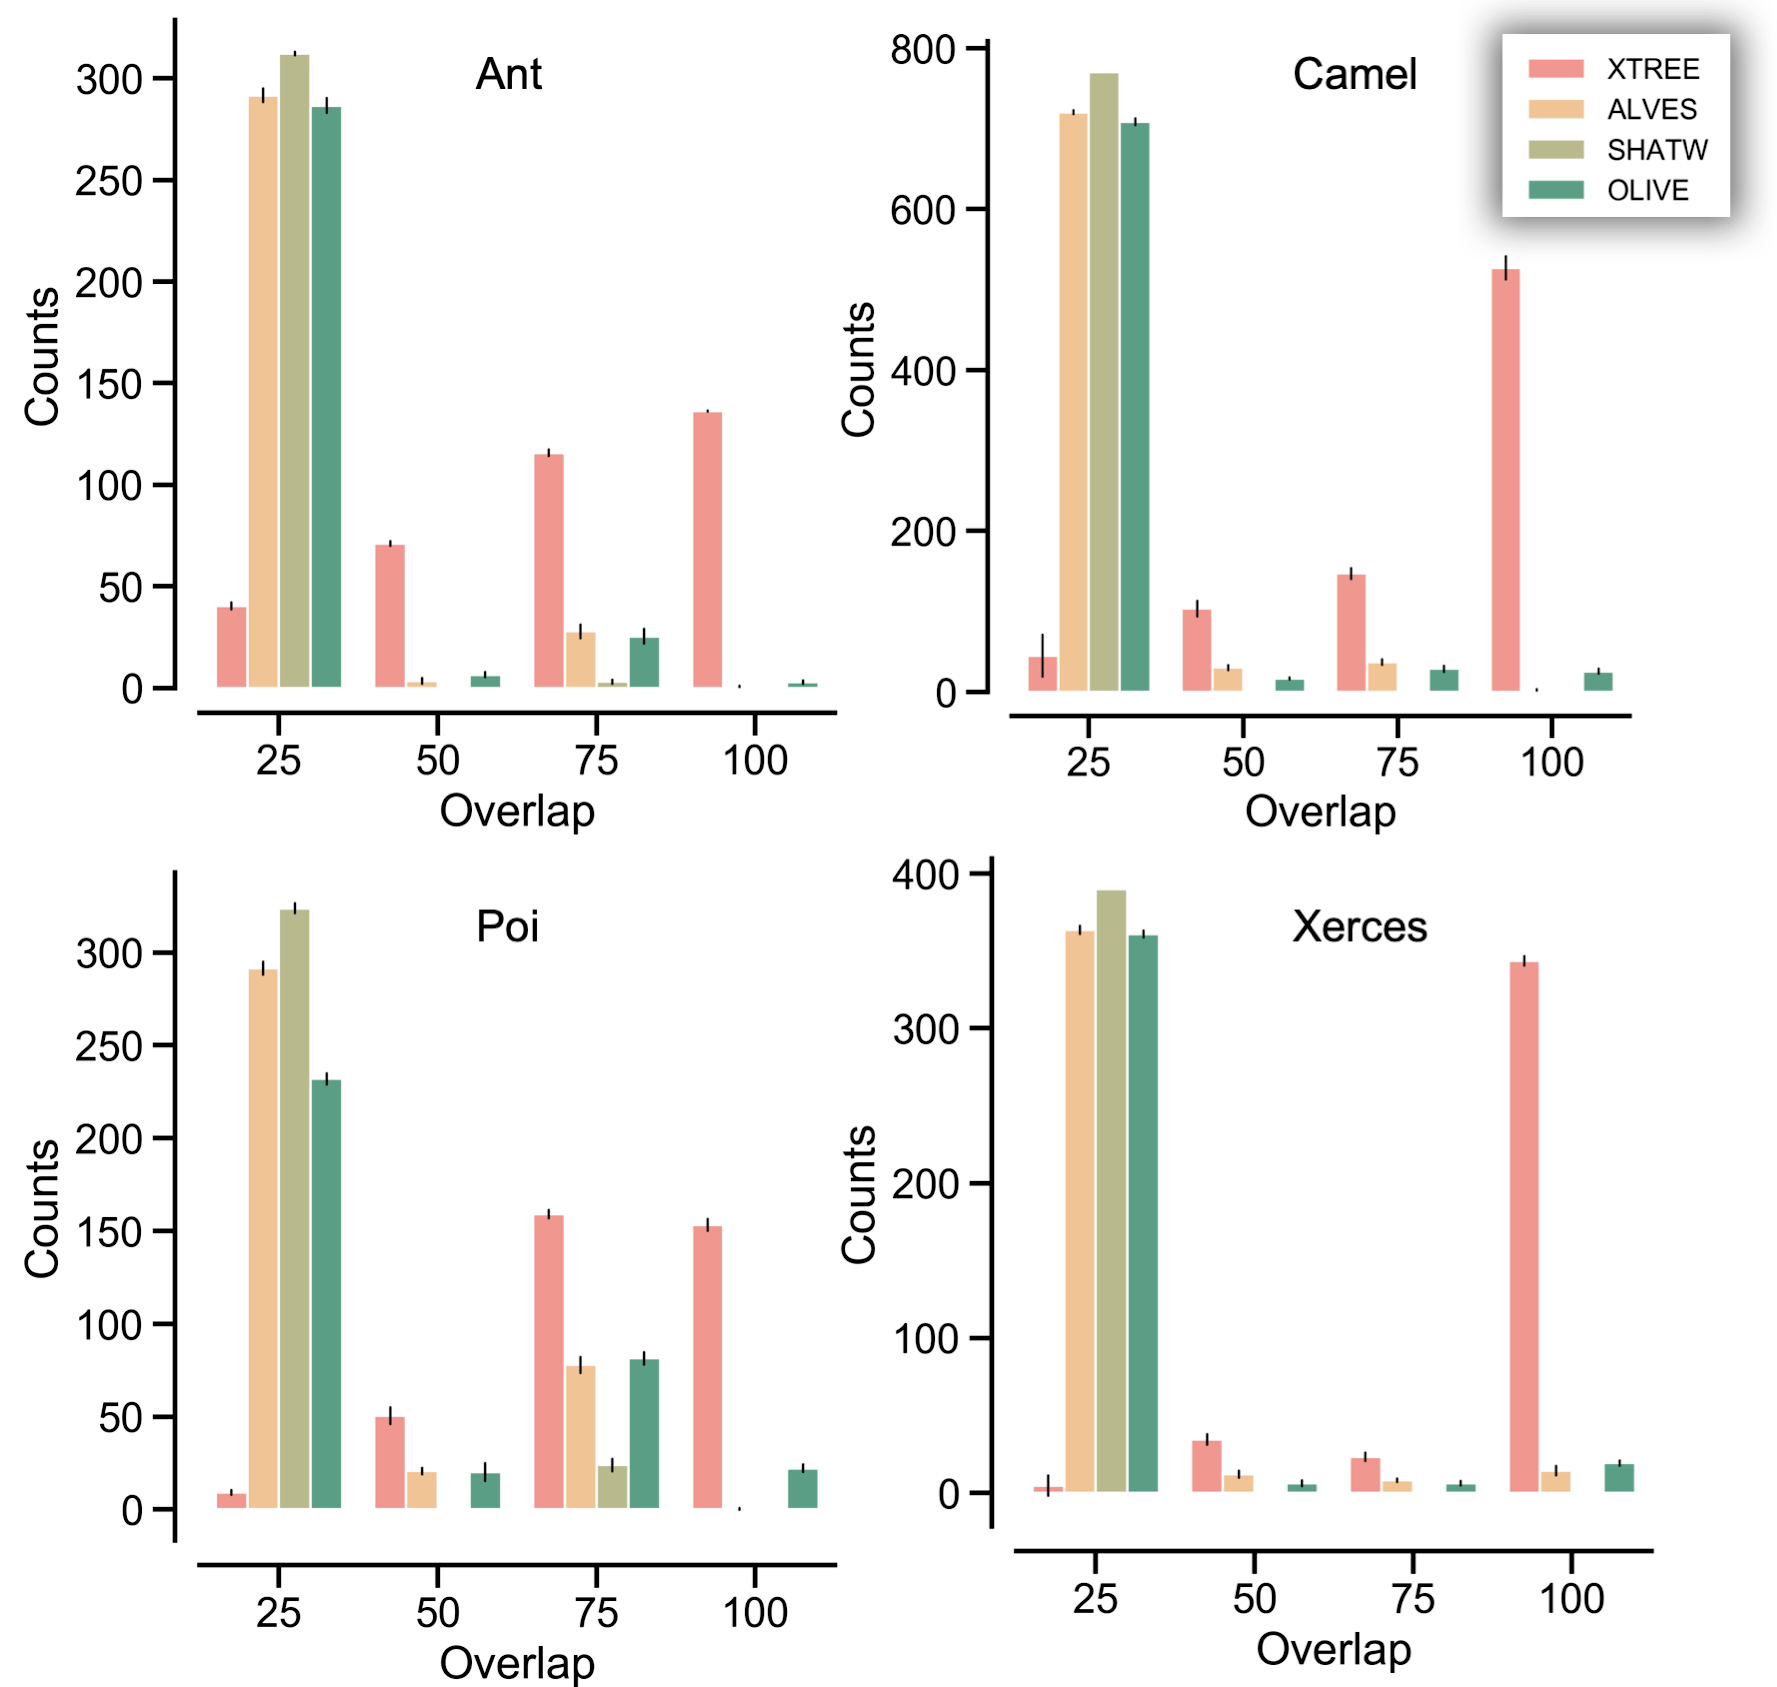
\includegraphics[width=0.75\linewidth]{rq1.png}
\caption{A count of number of test instances where the developer changes overlaps a planner recommendation. The overlaps (in the x-axis) are categorized into four ranges for every dataset (these are $0\leq~Overlap\leq25$, $26\leq~Overlap\leq50$, $51\leq~Overlap\leq75$, and $76\leq~Overlap\leq100$). For each of the overlap ranges, we count the the number of instances in the validation set where overlap between the planner's recommendation and the developers changes fell in that range. Note: \textit{Higher counts} for larger overlap is \textit{better}, e.g.,  $Count([75,100]) > Count([0,25))$ is considered better.}
\label{fig:results}
\end{figure}

To answer this question, we measure the \textit{overlap} between the planners' recommendations and the developer's actions. To measure this, we split the available data into training, testing, and validation sets. That is, given versions $\mathcal{V}_1, \mathcal{V}_2, \mathcal{V}_3....$, we, 
\be
\item {\em train} the planners on version $\mathcal{V}_1$; then 
\item {\em generate plans} using the planners for version $\mathcal{V}_2$;
\item then {\em validate} the effectiveness of those plans on $\mathcal{V}_2$ using the \ktest.
\ee
Then,  we repeat the process by training on $\mathcal{V}_2$, testing on $\mathcal{V}_3$, and validating on version $\mathcal{V}_4$, and so on. For each of these $\{train, test, validation\}$ sets, we measure the \textit{overlap} and categorize them into 4 ranges:
\bi
\item very little, i.e. $0-25\%$;
\item some, i.e. $26\%-50\%$;
\item more, i.e. $51\%-75\%$;
\item mostly, i.e. $76\%-100\%$.
\ei
\fig{results} shows the results of planning with several planners: XTREE, Alves, Shatnawi, and Oliveira. Note, for the sake of brevity, we illustrate results for 4 projects-- Ant, Camel, Poi, and Xerces. A full set set results for all projects are available at  \url{https://git.io/fjkNM}. 

We observe a clear dichotomy in our results. 
\bi
\item All outlier statistics based planners (i.e., those of Alves, Shatnawi, and Oliveira) have overlaps only in the range of 0\% to 25\%. This means that \textit{most of the developers actions did not match the recommendations proposed by these planners.}
\item In the case of XTREE, the largest number of files had an overlap of 76\% to 100\% and second largest was between 51\% to 75\%. This means that, in a majority of cases developers actions are 76\% to 100\% similar to XTREE's recommendations. At the very least, there was an 51\% similarity between XTREE's recommendations and developers actions.
\ei
We observe this trend in all 18 datasets-- XTREE significantly outperformed other threshold based planners in terms of the overlap between the plans and the actual actions undertaken by the developers. Note that reason the results are very negative about the methods of Alves, Shatnawi, Oliveira, et al. is because their recommendations would be very hard to operationalize (since those recommendations were seldom seen in the prior history of a project). Thus, our response to this research question can be summarized as follows:
\def\rot{\rotatebox}
\newcolumntype{a}{>{\columncolor{gr1}}r}
\newcolumntype{b}{>{\columncolor{gr2}}r}
\newcolumntype{c}{>{\columncolor{gr3}}r}
\newcolumntype{d}{>{\columncolor{gr4}}r}
\begin{figure}[!htbp]
\centering 
% \subfloat[subfig:plans][Defects Reduced. \textit{Higher defect reduction} for larger overlap is considered \textit{better}.]{
% \arrayrulecolor[gray]{0.5}
% \resizebox{\linewidth}{!}{
% \begin{tabular}{@{}l|rrra|rrrb|rrrc|rrrd}
%             \rowcolor{white}& \multicolumn{4}{c|}{$0\leq Overlap<25$}       & \multicolumn{4}{c|}{$25\leq Overlap<50$}       & \multicolumn{4}{c|}{$50\leq Overlap<75$}       & \multicolumn{4}{c}{$75\leq Overlap\leq100$}      \bigstrut \\ \hline
%             & \rot{90}{ALVES} & \rot{90}{OLIVE} & \rot{90}{SHATW~~} & \cellcolor{white}\rot{90}{XTREE} & \rot{90}{ALVES} & \rot{90}{OLIVE} & \rot{90}{SHATW~~} & \cellcolor{white}\rot{90}{XTREE} & \rot{90}{ALVES} & \rot{90}{OLIVE} & \rot{90}{SHATW~~} & \cellcolor{white}\rot{90}{XTREE} & \rot{90}{ALVES} & \rot{90}{OLIVE} & \rot{90}{SHATW~~} & \cellcolor{white}\rot{90}{XTREE} \bigstrut \\ \hline
% ant-1      & 3  & 2  & 13  & 13 & 6  & 7  & 3   & 33  & 1  & 2  & 0  & 27  & 2  & 3   & 0 & 62  \bigstrut \\
% ant-2      & 0  & 1  & 0   & 6  & 6  & 5  & 0   & 42  & 0  & 2  & 0  & 27  & 0  & 0   & 0 & 124 \bigstrut \\
% ant-3      & 10 & 6  & 22  & 18 & 16 & 15 & 1   & 71  & 2  & 5  & 0  & 47  & 0  & 1   & 0 & 108 \bigstrut \\ \hline
% camel-1    & 17 & 8  & 76  & 29 & 22 & 25 & 0   & 90  & 28 & 10 & 0  & 52  & 17 & 38  & 0 & 226 \bigstrut \\
% camel-2    & 9  & 3  & 36  & 25 & 21 & 17 & 0   & 109 & 18 & 11 & 0  & 69  & 0  & 18  & 0 & 439 \bigstrut \\ \hline
% ivy-1      & 1  & 1  & 1   & 4  & 0  & 0  & 0   & 10  & 0  & 0  & 0  & 5   & 0  & 0   & 0 & 12  \bigstrut \\ \hline
% jedit-1    & 9  & 5  & 13  & 9  & 7  & 6  & 8   & 35  & 5  & 7  & 0  & 39  & 0  & 3   & 0 & 136 \bigstrut \\
% jedit-2    & 14 & 7  & 28  & 24 & 10 & 14 & 1   & 77  & 4  & 2  & 0  & 36  & 0  & 2   & 0 & 107 \bigstrut \\ 
% jedit-3    & 14 & 10 & 18  & 30 & 4  & 6  & 1   & 67  & 1  & 1  & 0  & 28  & 0  & 1   & 0 & 70  \bigstrut \\ \hline
% log4j-1    & 2  & 0  & 5   & 1  & 1  & 3  & 0   & \cellcolor{white}7   & 1  & 0  & 0  & \cellcolor{white}3   & 0  & 1   & 0 & \cellcolor{white}8   \bigstrut \\ \hline
% lucene-1   & 8  & 2  & 21  & 6  & 17 & 17 & 19  & 36  & 13 & 5  & 0  & 17  & 1  & 15  & 0 & \cellcolor{white}57  \bigstrut \\ \hline
% poi-1      & 0  & 0  & 1   & \cellcolor{white}0  & 0  & 0  & 5   & \cellcolor{white}0   & 6  & 0  & 0  & \cellcolor{white}2   & 0  & 6   & 0 & \cellcolor{white}81  \bigstrut \\
% poi-2      & 49 & 2  & 78  & 4  & 32 & 72 & 18  & 135 & 15 & 12 & 0  & 27  & 0  & 16  & 0 & 87  \bigstrut \\ \hline
% velocity-1 & 9  & 2  & 51  & 2  & 26 & 12 & 0   & 25  & 11 & 15 & 0  & 39  & 4  & 24  & 0 & 90  \bigstrut \\ \hline
% xalan-1    & 4  & 2  & 22  & 6  & 27 & 19 & 105 & \cellcolor{white}43  & 70 & 21 & 13 & 60  & 38 & 103 & 0 & 409 \bigstrut \\
% xalan-2    & 7  & 0  & 110 & \cellcolor{white}0  & 63 & 18 & 0   & 38  & 51 & 53 & 0  & 102 & 4  & 56  & 0 & \cellcolor{white}83  \bigstrut \\ \hline
% xerces-1   & 2  & 1  & 23  & 2  & 6  & 3  & 0   & \cellcolor{white}11  & 9  & 3  & 0  & 17  & 7  & 18  & 0 & 305 \bigstrut \\
% xerces-2   & 0  & 0  & 7   & \cellcolor{white}0  & 1  & 1  & 0   & \cellcolor{white}3   & 6  & 2  & 0  & \cellcolor{white}6   & 1  & 6   & 0 & \cellcolor{white}117  
% \end{tabular}}
% \label{subfig:rq2_dec}}\\
% \subfloat[subfig:plans][Defects Increased. In comparison to defects reduced in \fig{rq2}(a) above, we would like to have as little defects increased as possible.]{
% \arrayrulecolor[gray]{0.5}
% \resizebox{\linewidth}{!}{
% \begin{tabular}{@{}l|rrra|rrrb|rrrc|rrrd}
%             \rowcolor{white}& \multicolumn{4}{c|}{$0\leq Overlap<25$}       & \multicolumn{4}{c|}{$25\leq Overlap<50$}       & \multicolumn{4}{c|}{$50\leq Overlap<75$}       & \multicolumn{4}{c}{$75\leq Overlap\leq100$}      \bigstrut \\ \hline
%             & \rot{90}{ALVES} & \rot{90}{OLIVE} & \rot{90}{SHATW~~} & \cellcolor{white}\rot{90}{XTREE} & \rot{90}{ALVES} & \rot{90}{OLIVE} & \rot{90}{SHATW~~} & \cellcolor{white}\rot{90}{XTREE} & \rot{90}{ALVES} & \rot{90}{OLIVE} & \rot{90}{SHATW~~} & \cellcolor{white}\rot{90}{XTREE} & \rot{90}{ALVES} & \rot{90}{OLIVE} & \rot{90}{SHATW~~} & \cellcolor{white}\rot{90}{XTREE} \bigstrut \\ \hline
% ant-1      & 15  & 15  & 15  & 1  & 0  & 0  & 0  & 10 & 0  & 0  & 0 & 2  & 0 & 0  & 0 & 4   \bigstrut\\
% ant-2      & 59  & 58  & 63  & 9  & 4  & 4  & 0  & 33 & 0  & 0  & 0 & 11 & 0 & 0  & 0 & 20  \bigstrut\\
% ant-3      & 66  & 64  & 69  & 22 & 4  & 7  & 0  & 38 & 0  & 0  & 0 & 15 & 0 & 0  & 0 & 10  \bigstrut\\\hline
% camel-1    & 29  & 28  & 36  & 10 & 5  & 5  & 0  & 11 & 2  & 2  & 0 & 6  & 0 & 0  & 0 & 14  \bigstrut\\
% camel-2    & 102 & 97  & 112 & 5  & 10 & 9  & 0  & 26 & 4  & 3  & 0 & 17 & 0 & 4  & 0 & 74  \bigstrut\\\hline
% ivy-1      & 6   & 6   & 6   & 1  & 0  & 0  & 0  & 3  & 0  & 0  & 0 & 2  & 0 & 0  & 0 & 0   \bigstrut\\\hline
% jedit-1    & 37  & 33  & 37  & 3  & 3  & 5  & 2  & 20 & 1  & 1  & 0 & 11 & 0 & 1  & 0 & 12  \bigstrut\\
% jedit-2    & 14  & 12  & 15  & 2  & 1  & 2  & 0  & 8  & 0  & 0  & 0 & 2  & 0 & 0  & 0 & 4   \bigstrut\\
% jedit-3    & 3   & 2   & 3   & 1  & 0  & 0  & 0  & 1  & 0  & 0  & 0 & 1  & 0 & 0  & 0 & 0   \bigstrut\\\hline
% log4j-1    & 68  & 66  & 73  & 1  & 3  & 4  & 1  & \cellcolor{white}14 & 3  & 2  & 0 & \cellcolor{white}13 & 0 & 2  & 0 & \cellcolor{white}47 \bigstrut\\\hline
% lucene-1   & 75  & 72  & 85  & 3  & 17 & 10 & 10 & 30 & 7  & 5  & 0 & 11 & 0 & 9  & 0 & \cellcolor{white}54 \bigstrut\\\hline
% poi-1      & 189 & 186 & 190 & \cellcolor{white}1  & 3  & 2  & 6  & \cellcolor{white}7  & 5  & 1  & 0 & \cellcolor{white}5  & 0 & 6  & 0 & \cellcolor{white}182 \bigstrut\\
% poi-2      & 84  & 78  & 87  & 4  & 8  & 9  & 2  & 23 & 0  & 2  & 0 & 11 & 0 & 0  & 0 & 58 \bigstrut\\\hline
% velocity-1 & 15  & 13  & 21  & 1  & 1  & 2  & 4  & 3  & 4  & 1  & 0 & 3  & 1 & 4  & 0 & 14 \bigstrut\\\hline
% xalan-1    & 144 & 142 & 152 & 2  & 15 & 9  & 21 & \cellcolor{white}46 & 13 & 8  & 6 & 33 & 4 & 13 & 0 & 101 \bigstrut\\
% xalan-2    & 460 & 452 & 506 & \cellcolor{white}27 & 26 & 5  & 0  & 25 & 35 & 33 & 0 & 87 & 0 & 18 & 0 & \cellcolor{white}388\bigstrut\\\hline
% xerces-1   & 49  & 47  & 52  & 0  & 1  & 2  & 0  & \cellcolor{white}10 & 1  & 1  & 0 & 11 & 0 & 0  & 0 & 34  \bigstrut\\
% xerces-2   & 163 & 161 & 169 & \cellcolor{white}4  & 6  & 5  & 0  & \cellcolor{white}14 & 1  & 2  & 0 & \cellcolor{white}9  & 0 & 1  & 0 & \cellcolor{white}146
% \end{tabular}}
% \label{fig:rq2_inc}
% }
\subfloat[Defects Reduced]{
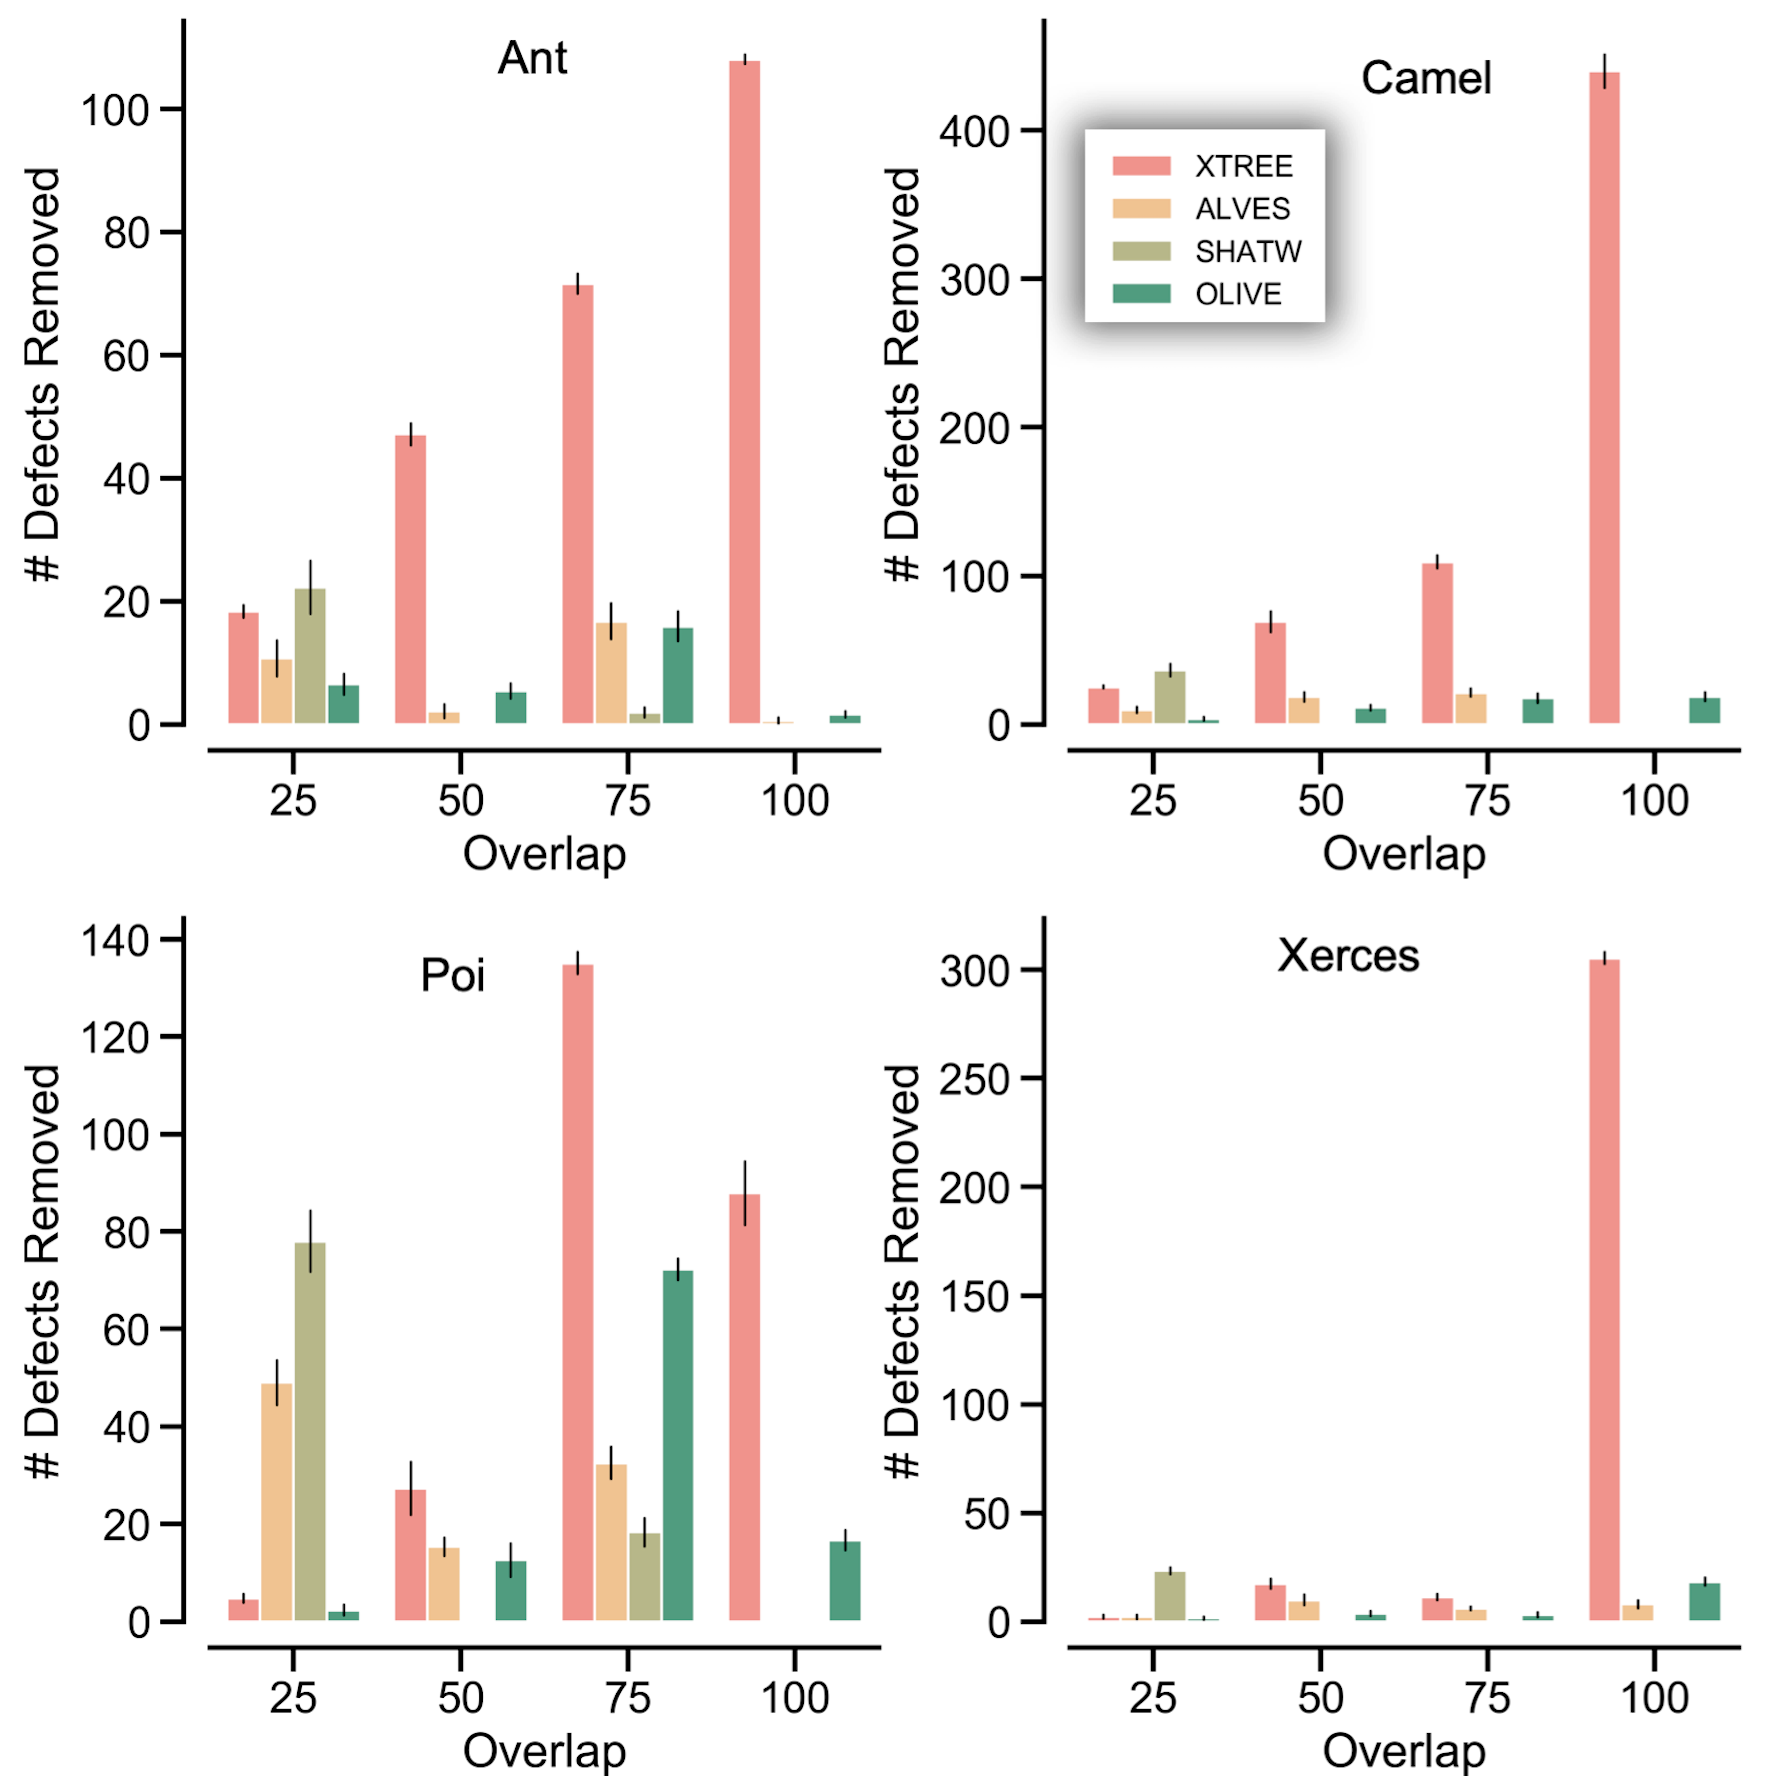
\includegraphics[width=0.75\linewidth]{rq2_1.png}
\label{fig:rq2_a}}\\~\hrule~
\subfloat[Defects Increased]{
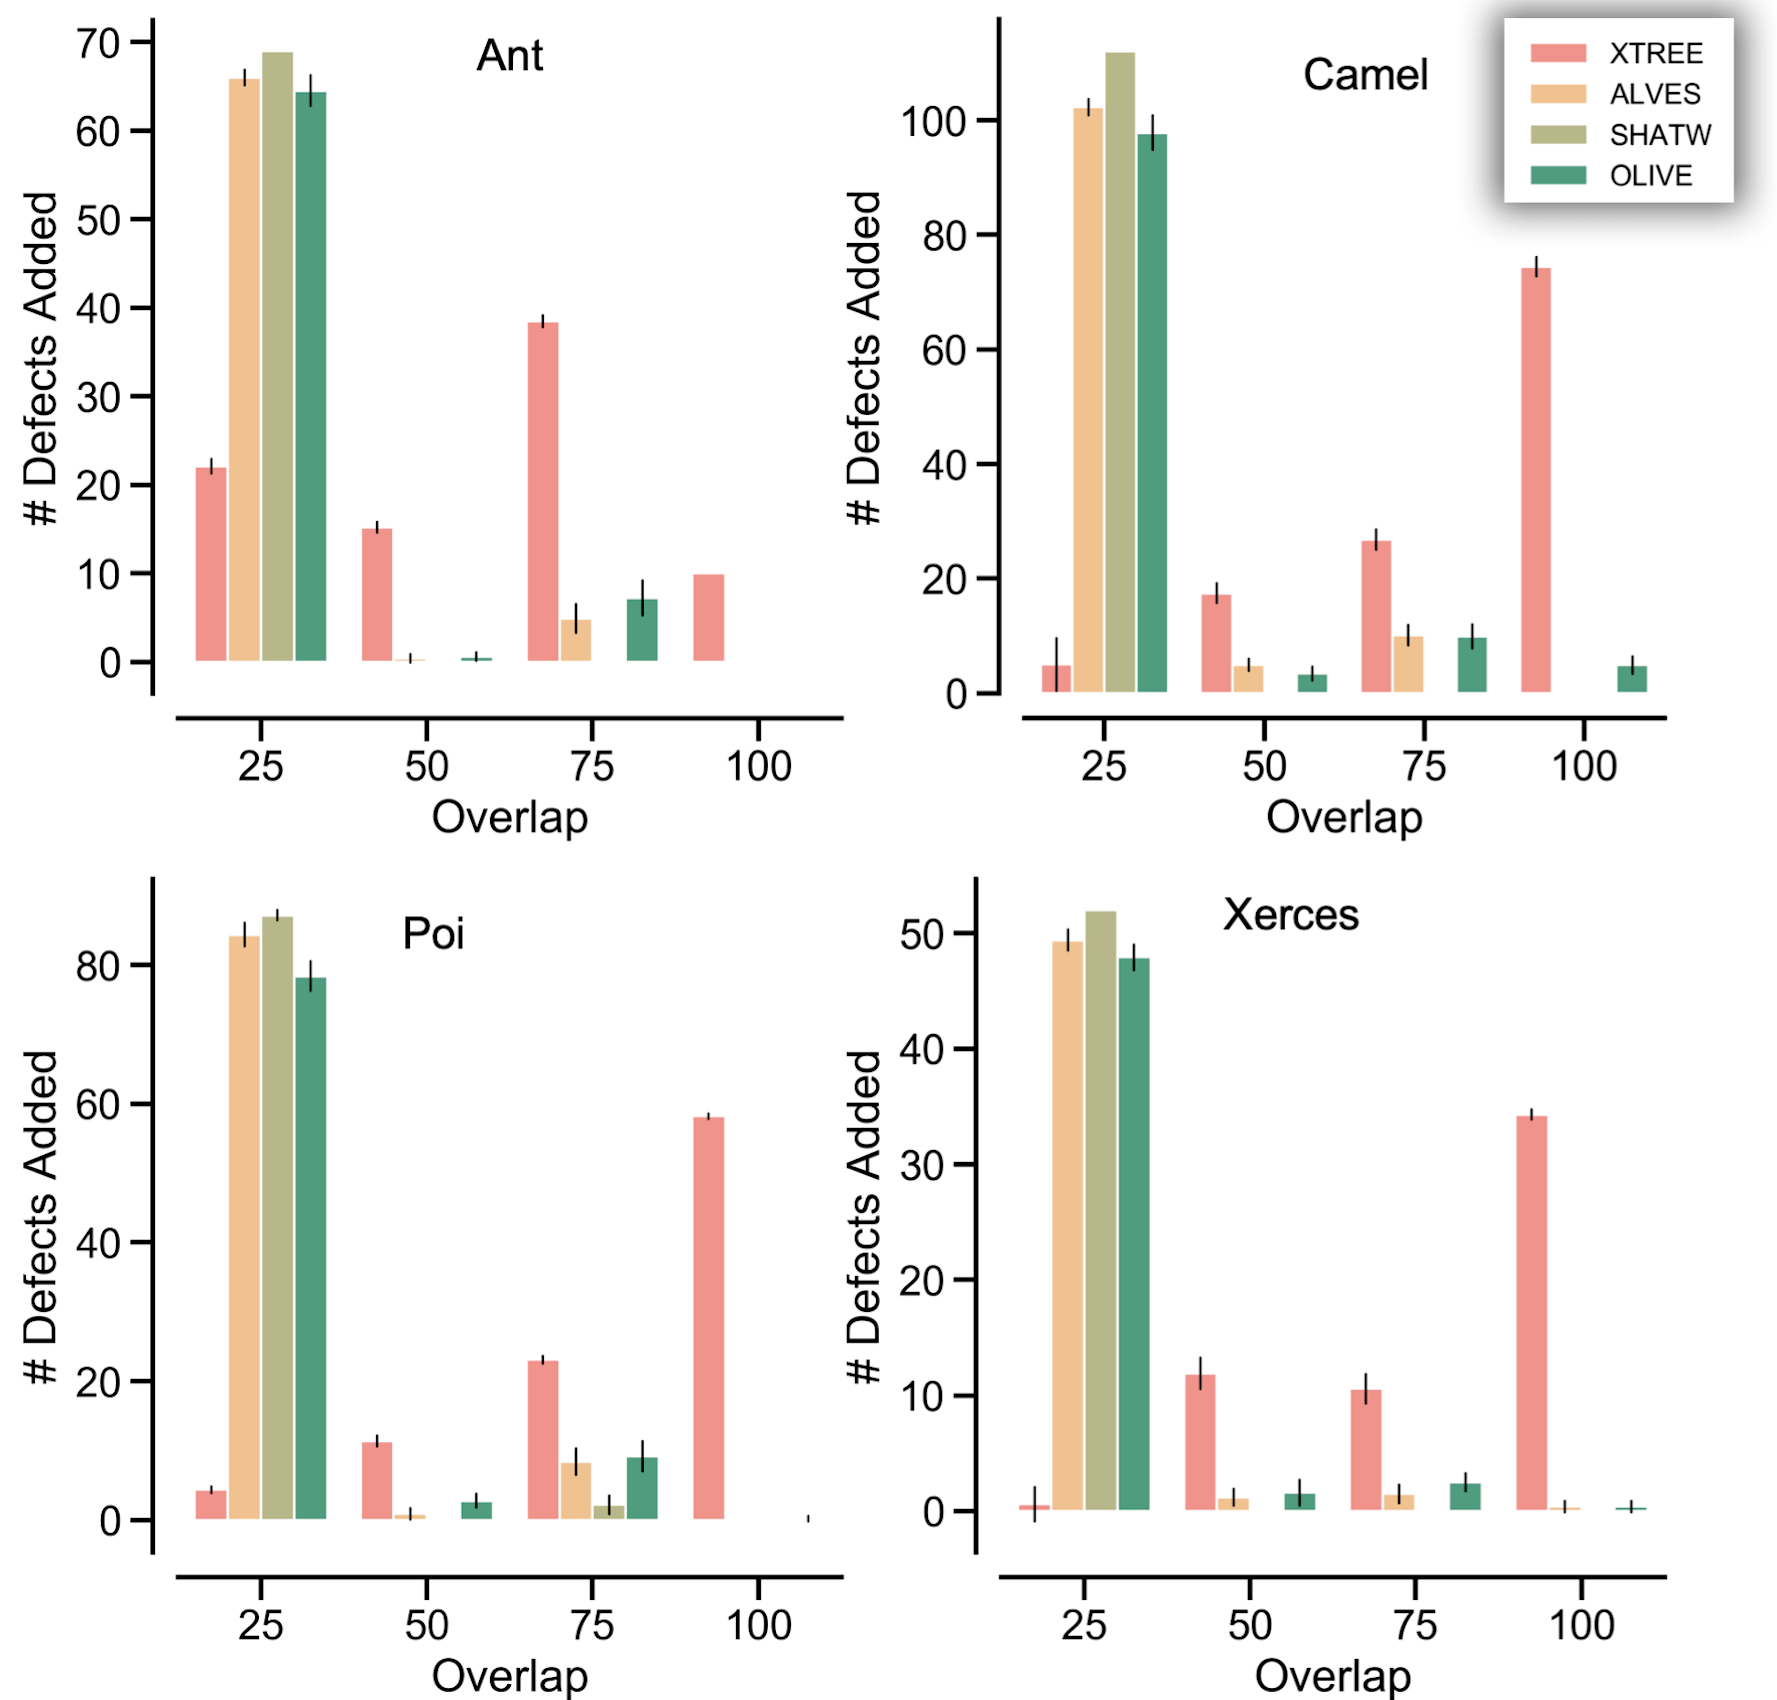
\includegraphics[width=0.75\linewidth]{rq2_2.png}
\label{fig:rq2_b}}
\caption{A count of total number \textit{defects reduced} and \textit{defects increased} as a result each planners' recommendations. The overlaps are again categorized into four ranges for every dataset (denoted by $min\leq~Overlap<max$). For each of the overlap ranges, we count the total number of \textit{defects reduced} and \textit{defects increased} in the validation set for the classes that were defective in the test set as a result of overlap between the planner's recommendation and the developers changes that fell in the given range}
\label{fig:rq2}
\end{figure}

\result{XTREE significantly outperforms all the other outlier statistics based planners. Further, in all the projects studied here, most of the developer actions to fix defects in a file has as 76\%--100\% overlap with the recommendations offered by XTREE.}

\subsection*{{\bf RQ2: Do planners' recommendation lead to reduction in defects?}}


In the previous research question measured the extent to which a planner's recommendations matched the actions taken by developers to fix defects in their files. But, the existence of a high overlap in most files does not necessarily mean that the defects are actually reduced. Likewise, it is also conceivable that that defects are added due to other actions the developer took during their development. Thus, it is important to ask how many defects are reduced, and how many are added, in response to larger overlap with the planners' recommendations.

Our experimental methodology to answer this research question is as follows: 
\bi
\item Like before, we measure the \textit{overlap} between the planners' recommendations developers' actions. \item Next, we plot the aggregate number defects reduced and in file with overlap values ranging from 0\% to 100\% in bins of size 25\% (for ranges of $0-25\%$, $26-50\%$, $51-75\%$, and $76-100\%$). 
\ei
Similar to RQ1, we compare XTREE with three other outlier statistics based planners of Alves et al., Shatnawi, and Oliveira, for the overall number of defects reduced and number of defects added. We prefer planners that have a large number defects reduced for higher overlap ranges are considered better.

\fig{rq2} shows the results of planning with several planners: XTREE, Alves, Shatnawi, and Oliveira. Note that, similar to the previous research question, we only illustrate results for 4 projects-- Ant, Camel, Poi, and Xerces. A full set of results for RQ2 for all projects are available at \url{https://git.io/fjIvG}. 

We make the following observations from in our results: 
\be
\item \textit{Defects Decreased}: \fig{rq2}\protect\subref{fig:rq2_a} plots the number of defects \textit{removed} in files with various overlap ranges. It is desirable to see larger defects removed with larger overlap. We note that:
\bi
\item When compared to other planners, the number of defects removed as a result of recommendations obtained by XTREE is significantly larger. This trend was noted in all the projects we studied here.
\item In the cases of Ant, Camel, and Xerces there are large number of defect reduced when the overlap lies between 76\% and 100\%. Poi is an exception-- here, we note that the largest number of defects are removed when the overlap is between 51\% and 75\%. 
\ei

\item \textit{Defects Increased}: \fig{rq2}\protect\subref{fig:rq2_b} plots the number of defects \textit{added} in files with various overlap ranges. It is desirable to see lower number of defects added with larger overlap. We note that: 
\bi
\item When compared to other planners, the number of defects added as a result of recommendations obtained by XTREE is comparatively larger. This trend was noted in all the projects we studied here. This is to be expected since, developers actions seldom match the recommendations of these other planners. 

\item In all the cases the number of defects removed was significantly larger than the number of defects added. For example, in the case of Camel, 420+ defects were removed at 76\% -- 100\% overlap and about 70 defects were added (i.e., 6$\times$ more defects were removed than added). Likewise, in the case of Xerces, over 300 defects were removed and only about 30 defects were added (i.e., 10$\times$ more defects were removed than added).
\ei
\ee

The ratio of defects removed to the number of defects added is very important to asses. \fig{rq2_1} plots this ratio at 76\% -- 100\% overlap (it applied equally for the other overlap ranges as they have far fewer defects removed and added). From this chart, we note that out of 18 datasets, in 14 cases XTREE lead to a significant reduction in defects. For example, in the case of Ivy and Log4j, there were no defects added at all.

However, in 4 cases, there were more defects added than there were removed. Given the idiosyncrasies  of real world projects, we do not presume that developers will always take actions as suggested by a planner. This may lead to defects being increased, however, based on our results we notice that this is not a common occurrence.
In summary, our response to this research question is as follows:

\noindent\result{Plans  generated  by  XTREE  are  superior  to  other  outlier  statistics based  planners  in  all  10  projects.  Planning  with  XTREE  leads  to  the  far larger number of defects reduced as opposed to defects added in 9 out of 10 projects studied here.}
\begin{figure}[!tbp]
\centering 
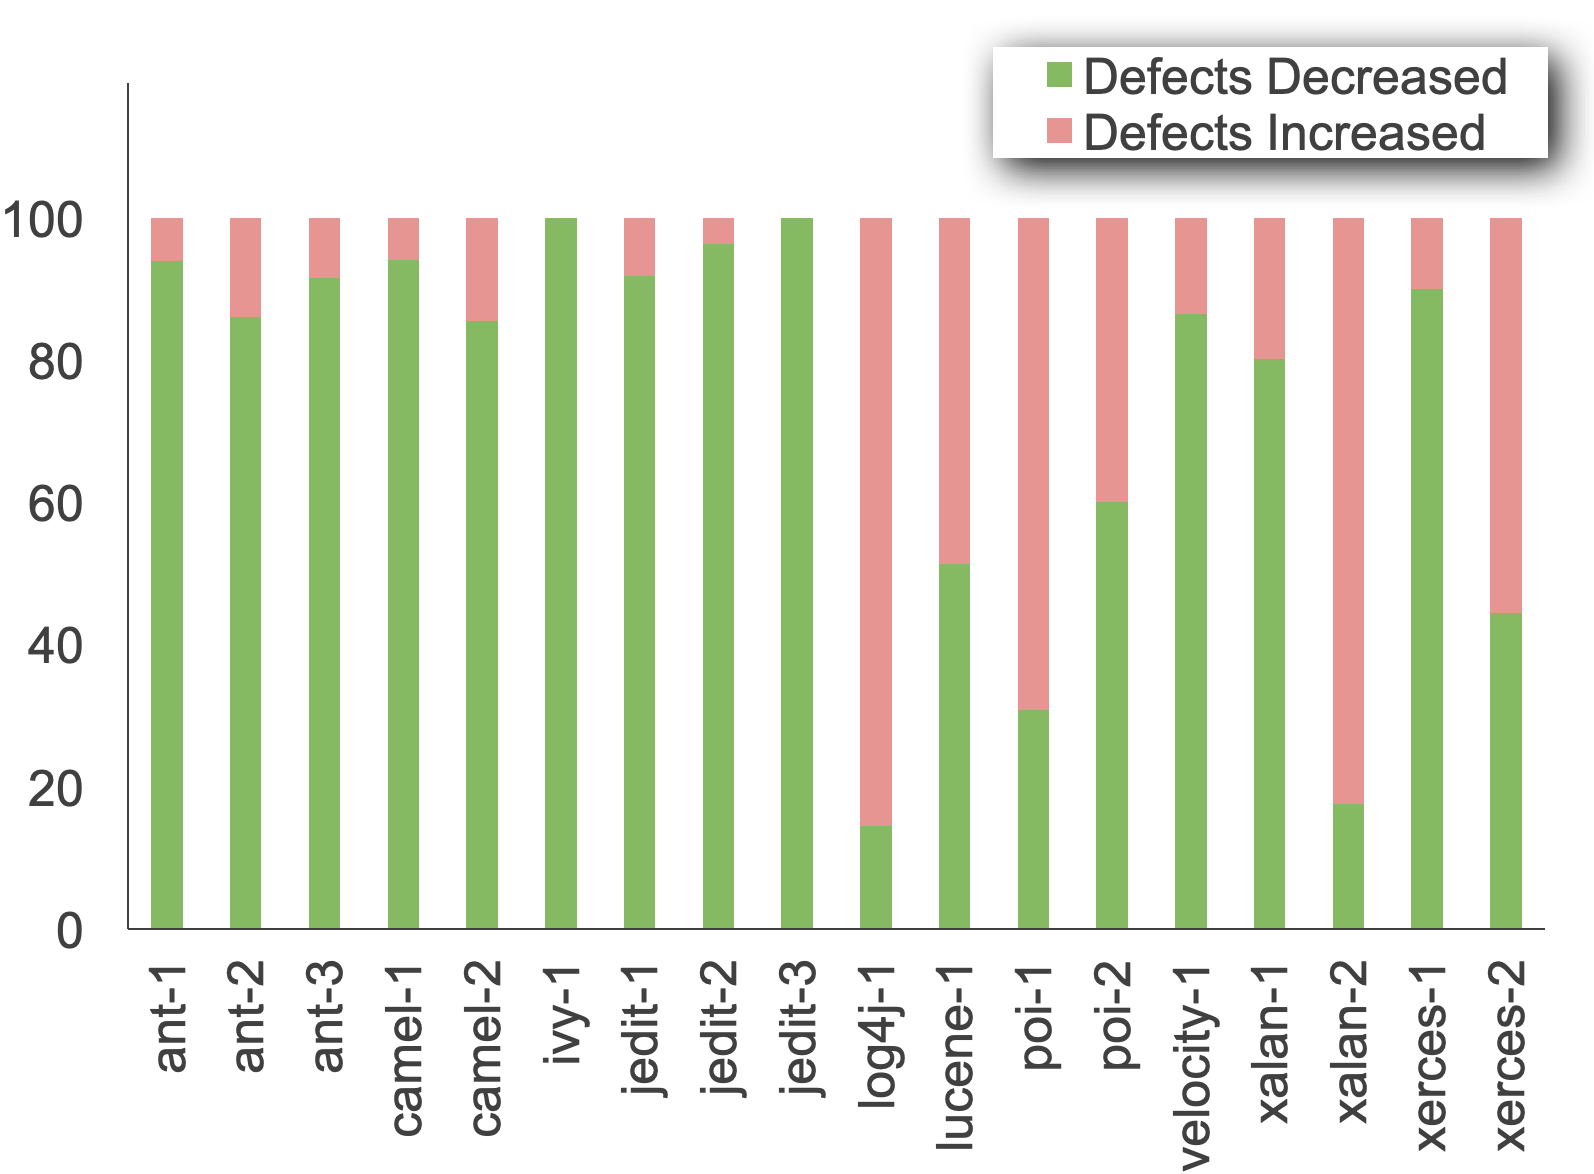
\includegraphics[width=0.75\linewidth]{rq2_3.png}
\caption{A count of total number \textit{defects reduced} and \textit{defects increased} as a result each planners' recommendations. The overlaps are again categorized into four ranges for every dataset (denoted by $min\leq~Overlap<max$). For each of the overlap ranges, we count the total number of \textit{defects reduced} and \textit{defects increased} in the validation set for the classes that were defective in the test set as a result of overlap between the planner's recommendation and the developers changes that fell in the given range}
\label{fig:rq2_1}
\end{figure}
\vspace{-0.4em}

\subsection*{{\bf RQ3: Are  cross-project  plans  generated  by  BELLTREE  as  effective  as  within-project plans of XTREE?}}
\def\rot{\rotatebox}
\begin{figure}[!htbp]
\centering 
\subfloat[subfig:plans][Defects Reduced. \textit{Higher defect reduction} for larger Overlap is considered \textit{better}.]{
\arrayrulecolor[gray]{0.5}
\resizebox{0.8\linewidth}{!}{
\begin{tabular}{@{}l|rrr|rrr|rrr|rrr}
            \rowcolor{white}& \multicolumn{3}{c|}{$[0, 25)$~~~~~~}       & \multicolumn{3}{c|}{$[25, 50)$~~~~~}       & \multicolumn{3}{c|}{$[50, 75)~~~~~$}       & \multicolumn{3}{c}{$[75, 100]$~~~~}       \bigstrut\\ \hline
            &  \rot{90}{RAND} & \rot{90}{XTREE} & \rot{90}{BELLTREE~~} & \rot{90}{RAND} & \rot{90}{XTREE} & \rot{90}{BELLTREE~~} & \rot{90}{RAND} & \rot{90}{XTREE} & \rot{90}{BELLTREE~~} & \rot{90}{RAND} & \rot{90}{XTREE} & \rot{90}{BELLTREE~~}  \bigstrut\\\hline
ant-1      & \cellcolor{gr1}13    & \cellcolor{gr1}13    & 12       & 3     & \cellcolor{gr2}33    & 19       & 0     & \cellcolor{gr4}27    & 10       & 0     & \cellcolor{gr4}62    & 54       \bigstrut\\

ant-2      & 0     & 6     & \cellcolor{gr1}13       & 0     & \cellcolor{gr2}42    & 33       & 0     & \cellcolor{gr4}27    & \cellcolor{gr4}27       & 0     & \cellcolor{gr4}124   & 61       \bigstrut\\

ant-3      & \cellcolor{gr1}22    & 18    & 6        & 1     & \cellcolor{gr2}71    & 42       & 0     & \cellcolor{gr4}47    & 27       & 0     & 108   & \cellcolor{gr4}124      \bigstrut\\ \hline

camel-1    & \cellcolor{gr1}76    & 29    & 10       & 0     & \cellcolor{gr2}90    & 30       & 0     & \cellcolor{gr3}52    & 20       & 0     & \cellcolor{gr4}226   & 98       \bigstrut\\

camel-2    & \cellcolor{gr1}36    & 25    & 30       & 0     & \cellcolor{gr2}109   & 100      & 0     & \cellcolor{gr3}69    & 68       & 0     & \cellcolor{gr4}439   & 277      \bigstrut\\ \hline

ivy-1      & 1     & 4     & \cellcolor{gr1}12       & 0     & 10    & \cellcolor{gr2}42       & 0     & 5     & \cellcolor{gr3}13       & 0     & 12    & \cellcolor{gr4}25       \bigstrut\\ \hline

jedit-1    & \cellcolor{gr1}13    & 9     & 11       & 8     & 35    & \cellcolor{gr2}44       & 0     & 39    & \cellcolor{gr3}50       & 0     & \cellcolor{gr4}136   & 108      \bigstrut\\

jedit-2    & \cellcolor{gr1}28    & 24    & 10       & 1     & \cellcolor{gr2}77    & 34       & 0     & 36    & \cellcolor{gr3}39       & 0     & 107   &\cellcolor{gr4} 135      \bigstrut\\

jedit-3    & 18    & \cellcolor{gr1}30    & 28       & 1     & 67    & \cellcolor{gr2}75       & 0     & 28    & \cellcolor{gr3}35       & 0     & 70    & \cellcolor{gr4}106      \bigstrut\\ \hline

log4j-1    & \cellcolor{gr1}5     & 1     & 0        & 0     & 7     & \cellcolor{gr2}14       & 0     & 3     & \cellcolor{gr3}8        & 0     & 8     & \cellcolor{gr4}50       \bigstrut\\ \hline

poi-1      & 1     & 0     & \cellcolor{gr1}7        & 5     & 0     & \cellcolor{gr2}80       & 0     & 2     & \cellcolor{gr3}19       & 0     & 81    & \cellcolor{gr4}90       \bigstrut\\

poi-2      & \cellcolor{gr1}78    & 4     & 0        & 18    & \cellcolor{gr2}135   & 0        & 0     & \cellcolor{gr3}27    & 2        & 0     & \cellcolor{gr4}87    & 83       \bigstrut\\ \hline

velocity-1 & \cellcolor{gr1}51    & 2     & 6        & 0     & \cellcolor{gr2}25    & 15       & 0     & \cellcolor{gr3}39    & 32       & 0     & \cellcolor{gr4}90    & 48       \bigstrut\\ \hline

xalan-1    & \cellcolor{gr1}22    & 6     & 2        & \cellcolor{gr2}105   & 43    & 51       & 13    & 60    & \cellcolor{gr3}66       & 0     & \cellcolor{gr4}409   & 230      \bigstrut\\

xalan-2    & \cellcolor{gr1}110   & 0     & 6        & 0     & 38    & \cellcolor{gr2}49       & 0     & \cellcolor{gr3}102   & 54       & 0     & 83    & \cellcolor{gr4}408      \bigstrut\\ \hline

xerces-1   & \cellcolor{gr1}23    & 2     & 11       & 0     & 11    & \cellcolor{gr2}13       & 0     & 17    & \cellcolor{gr3}24       & 0     & \cellcolor{gr4}305   & 49       \bigstrut\\

xerces-2   & \cellcolor{gr1}7     & 0     & 2        & 0     & 3     & \cellcolor{gr2}11       & 0     & 6     & \cellcolor{gr3}18       & 0     & 117   & \cellcolor{gr4}305     

\end{tabular}}
\label{fig:rq3_dec}}\\
\subfloat[subfig:plans][Defects Increased. In comparison to defects reduced in \fig{rq2}(a) above, we would like to have as little defects increased as possible.]{
\arrayrulecolor[gray]{0.5}
\resizebox{0.8\linewidth}{!}{
\begin{tabular}{@{}l|rrr|rrr|rrr|rrr}
            \rowcolor{white}& \multicolumn{3}{c|}{$[0, 25)$~~~~~~}       & \multicolumn{3}{c|}{$[25, 50)$~~~~~}       & \multicolumn{3}{c|}{$[50, 75)$~~~~~}       & \multicolumn{3}{c}{$[75, 100]$~~~~}       \bigstrut\\ \hline
            &  \rot{90}{RAND} & \rot{90}{XTREE} & \rot{90}{BELLTREE~~} & \rot{90}{RAND} & \rot{90}{XTREE} & \rot{90}{BELLTREE~~} & \rot{90}{RAND} & \rot{90}{XTREE} & \rot{90}{BELLTREE~~} & \rot{90}{RAND} & \rot{90}{XTREE} & \rot{90}{BELLTREE~~}  \bigstrut\\ \hline
ant-1      & 15  & \cellcolor{gr1}1  & \cellcolor{gr1}3 & 0  & \cellcolor{gr2}10 & \cellcolor{gr2}11 & 0 & \cellcolor{gr3}2  & \cellcolor{gr3}1  & 0 & 4   & \cellcolor{gr4}2   \bigstrut\\
ant-2      & 63  & 9  & \cellcolor{gr1}1 & 0  & 33 & \cellcolor{gr2}10 & 0 & 11 & \cellcolor{gr3}2  & 0 & 20  & \cellcolor{gr4}4   \bigstrut\\
ant-3      & 69  & 22 & \cellcolor{gr1}9 & 0  & 38 & \cellcolor{gr2}33 & 0 & 15 & 11 & 0 & \cellcolor{gr4}10  & 20  \bigstrut\\ \hline
camel-1    & 36  & 10 & \cellcolor{gr1}5 & 0  & \cellcolor{gr2}11 & 25 & 0 & \cellcolor{gr3}6  & 14 & 0 & \cellcolor{gr4}14  & 31  \bigstrut\\
camel-2    & 112 & \cellcolor{gr1}5  & \cellcolor{gr1}2 & 0  & 26 & \cellcolor{gr2}15 & 0 & 17 & \cellcolor{gr3}\cellcolor{gr3}9  & 0 & 74  & \cellcolor{gr4}15  \bigstrut\\ \hline
ivy-1      & 6   & \cellcolor{gr1}1  & \cellcolor{gr1}0 & 0  & \cellcolor{gr2}3  & \cellcolor{gr2}2  & 0 & \cellcolor{gr3}2  & \cellcolor{gr3}1  & 0 & 0   & 0   \bigstrut\\ \hline
jedit-1    & 37  & \cellcolor{gr1}3  & \cellcolor{gr1}2 & 2  & 20 & \cellcolor{gr2}10 & 0 & 11 & \cellcolor{gr3}6  & 0 & 12  & \cellcolor{gr4}6   \bigstrut\\
jedit-2    & 15  & \cellcolor{gr1}2  & \cellcolor{gr1}5 & 0  & \cellcolor{gr2}8  & 19 & 0 & \cellcolor{gr3}2  & 11 & 0 & \cellcolor{gr4}4   & 12  \bigstrut\\
jedit-3    & 3   & \cellcolor{gr1}1  & \cellcolor{gr1}1 & 0  & 1  & \cellcolor{gr2}0  & 0 & \cellcolor{gr3}1  & \cellcolor{gr3}1  & 0 & 0   & 0   \bigstrut\\ \hline
log4j-1    & 73  & \cellcolor{gr1}1  & \cellcolor{gr1}2 & 1  & 14 & \cellcolor{gr2}7  & 0 & 13 & \cellcolor{gr3}2  & 0 & 47  & \cellcolor{gr4}7   \bigstrut\\ \hline
poi-1      & 190 & \cellcolor{gr1}1  & \cellcolor{gr1}1 & 6  & 7  & \cellcolor{gr2}1  & 0 & 5  & \cellcolor{gr3}0  & 0 & 182 & \cellcolor{gr4}6   \bigstrut\\
poi-2      & 87  & 4  & \cellcolor{gr1}0 & 2  & 23 & \cellcolor{gr2}7  & 0 & 11 & \cellcolor{gr3}5  & 0 & \cellcolor{gr4}58  & 184 \bigstrut\\ \hline
velocity-1 & 21  & \cellcolor{gr1}1  & \cellcolor{gr1}4 & 4  & \cellcolor{gr2}3  & 14 & 0 & \cellcolor{gr3}3  & 17 & 0 & 14  & \cellcolor{gr4}10  \bigstrut\\ \hline
xalan-1    & 152 & \cellcolor{gr1}2  & \cellcolor{gr1}3 & 21 & 46 & \cellcolor{gr2}29 & 6 & 33 & \cellcolor{gr3}31 & 0 & \cellcolor{gr4}101 & 217 \bigstrut\\
xalan-2    & 506 & 27 & \cellcolor{gr1}3 & 0  & \cellcolor{gr2}25 & 48 & 0 & 87 & \cellcolor{gr3}32 & 0 & 388 & \cellcolor{gr4}101 \bigstrut\\ \hline
xerces-1   & 52  & \cellcolor{gr1}0  & \cellcolor{gr1}0 & 0  & 10 & \cellcolor{gr2}1  & 0 & 11 & \cellcolor{gr3}1  & 0 & \cellcolor{gr4}34  & 1   \bigstrut\\
xerces-2   & 169 & 4  & \cellcolor{gr1}0 & 0  & 14 & \cellcolor{gr2}11 & 0 & \cellcolor{gr3}9  & 12 & 0 & 146 & \cellcolor{gr4}34 
\end{tabular}}
\label{fig:rq3_inc}
}
\caption{A count of total number \textit{defects reduced} and \textit{defects increased} as a result each planners' recommendations. The overlaps are again categorized into four ranges for every dataset (denoted by $min\leq~Overlap<max$). For each of the Overlap ranges, we count the total number of \textit{defects reduced} and \textit{defects increased} in the validation set for the classes that were defective in the test set as a result of Overlap between the planner's recommendation and the developers changes that fell in the given range}
\label{fig:rq3}
\end{figure}

In the previous two research questions, we made an assumption that there are past releases that can be used to construct the planners. However, this may not always be the case. For new project, it is quite possible that there are not any historical data to construct the planners. In such cases, SE literature proposes the use of \textit{transfer learning}. In this paper, we leverage the so-called \textit{bellwether} effect to identify a bellwether project. Having done so, we construct a planner quite similar to XTREE with the exception that the training data comes from the bellwether project. This variant of our planner that uses the bellwether project is called the BELLTREE (see \tion{CPXTREE} for more details).

To answer this research question, we train XTREE on within-project data and generate plans for reducing the number of defects. We then compare this with plans derived from the bellwether data and BELLTREE. We hypothesized that since bellwethers have been demonstrated to be efficient in prediction tasks, learning from the bellwethers for a specific community of projects would produce performance scores comparable to within-project data. Our experimental methodology to answer this research question is as follows: 
\be
\item Like before, we measure the \textit{overlap} between the planners' recommendations developers' actions. 
\item Next, we tabulate the aggregate number defects reduced (\fig{rq3}\protect\subref{fig:rq3_dec}) and the number of defects increased (\fig{rq3}\protect\subref{fig:rq3_inc}) in files with overlap values ranging from 0\% to 100\% in bins of size 25\% (for ranges of $0-25\%$, $26-50\%$, $51-75\%$, and $76-100\%$). 
\ee

Similar to previous research questions, we compare XTREE with BELLTREE and a random oracle (RAND). We prefer planners that have a large number defects reduced for higher overlap ranges and planner that have lower number of defects added are are considered better.

We make the following observations from in our results: 
\be
\item \textit{Defects Decreased}: \fig{rq2}\protect\subref{fig:rq2_a} plots the number of defects \textit{removed} in files with various overlap ranges. It is desirable to see larger defects removed with larger overlap. We note that:
\bi
\item When compared to other planners, the number of defects removed as a result of recommendations obtained by XTREE is significantly larger. This trend was noted in all the projects we studied here.
\item In the cases of Ant, Camel, and Xerces there are large number of defect reduced when the overlap lies between 76\% and 100\%. Poi is an exception-- here, we note that the largest number of defects are removed when the overlap is between 51\% and 75\%. 
\ei

\item \textit{Defects Increased}: \fig{rq2}\protect\subref{fig:rq2_b} plots the number of defects \textit{added} in files with various overlap ranges. It is desirable to see lower number of defects added with larger overlap. We note that: 
\bi
\item When compared to other planners, the number of defects added as a result of recommendations obtained by XTREE is comparatively larger. This trend was noted in all the projects we studied here. This is to be expected since, developers actions seldom match the recommendations of these other planners. 

\item In all the cases the number of defects removed was significantly larger than the number of defects added. For example, in the case of Camel, 420+ defects were removed at 76\% -- 100\% overlap and about 70 defects were added (i.e., 6$\times$ more defects were removed than added). Likewise, in the case of Xerces, over 300 defects were removed and only about 30 defects were added (i.e., 10$\times$ more defects were removed than added).
\ei
\ee

The ratio of defects removed to the number of defects added is very important to asses. \fig{rq2_1} plots this ratio at 76\% -- 100\% overlap (it applied equally for the other overlap ranges as they have far fewer defects removed and added). From this chart, we note that out of 18 datasets, in 14 cases XTREE lead to a significant reduction in defects. For example, in the case of Ivy and Log4j, there were no defects added at all.

However, in 4 cases, there were more defects added than there were removed. Given the idiosyncrasies  of real world projects, we do not presume that developers will always take actions as suggested by a planner. This may lead to defects being increased, however, based on our results we notice that this is not a common occurrence.


In summary, our response to this research question is as follows:\\


\result{The effectiveness of BELLTREE and XTREE are similar. If within-project data is available, we recommend using XTREE. If not, BELLTREE is a viable alternative.}

% \subsection*{{\bf RQ4: How many changes do the planners propose?}}
% % \begin{figure*}[t!]
% \resizebox{\linewidth}{!}{
% \begin{tabular}{l|llll|llll|llll|llll|llll|llll|llll|llll|llll}
%         & \multicolumn{4}{c|}{Ant}       & \multicolumn{4}{c|}{Ivy}       & \multicolumn{4}{c|}{Camel}     & \multicolumn{4}{c|}{Xerces}    & \multicolumn{4}{c|}{Velocity}  & \multicolumn{4}{c|}{Xalan}     & \multicolumn{4}{c|}{Poi}       & \multicolumn{4}{c|}{Log4j}     & \multicolumn{4}{c}{Jedit}     \bigstrut[b]\\\hline
% \begin{sideways}Metrics\end{sideways} & \begin{sideways}XTREE\end{sideways} & \begin{sideways}Alves\end{sideways} & \begin{sideways}Shatnawi~~~\end{sideways} & \begin{sideways}Oliveira\end{sideways} & \begin{sideways}XTREE\end{sideways} & \begin{sideways}Alves\end{sideways} & \begin{sideways}Shatnawi~~~\end{sideways} & \begin{sideways}Oliveira\end{sideways} & \begin{sideways}XTREE\end{sideways} & \begin{sideways}Alves\end{sideways} & \begin{sideways}Shatnawi~~~\end{sideways} & \begin{sideways}Oliveira\end{sideways} & \begin{sideways}XTREE\end{sideways} & \begin{sideways}Alves\end{sideways} & \begin{sideways}Shatnawi~~~\end{sideways} & \begin{sideways}Oliveira\end{sideways} & \begin{sideways}XTREE\end{sideways} & \begin{sideways}Alves\end{sideways} & \begin{sideways}Shatnawi~~~\end{sideways} & \begin{sideways}Oliveira\end{sideways} & \begin{sideways}XTREE\end{sideways} & \begin{sideways}Alves\end{sideways} & \begin{sideways}Shatnawi~~~\end{sideways} & \begin{sideways}Oliveira\end{sideways} & \begin{sideways}XTREE\end{sideways} & \begin{sideways}Alves\end{sideways} & \begin{sideways}Shatnawi~~~\end{sideways} & \begin{sideways}Oliveira\end{sideways} & \begin{sideways}XTREE\end{sideways} & \begin{sideways}Alves\end{sideways} & \begin{sideways}Shatnawi~~~\end{sideways} & \begin{sideways}Oliveira\end{sideways} & \begin{sideways}XTREE\end{sideways} & \begin{sideways}Alves\end{sideways} & \begin{sideways}Shatnawi~~~\end{sideways} & \begin{sideways}Oliveira\end{sideways} \bigstrut\\\hline
% wmc     &    & 89    & 100   & 94    &    & 94    & 100   & 94    &    & 94    & 100   & 92    &    & 87    & 100   & 94    &    & 84    & 100   & 92    &    & 72    & 100   & 90    &    & 98    & 91    & 94    &    & 80    & 100   & 93    &    & 87    & 69    & 94    \bigstrut[t]\\
% dit     &    & 47    & 100   & 66    &    & 100   & 28    & 49    &    & 40    &    & 62    & 16    & 90    & 87    & 52    &    & 67    & 100   & 44    &    & 59    & 77    & 67    &    & 50    & 100   & 50    &    & 16    & 100   & 46    &    & 69    & 100   & 66    \\
% noc     &    &    & 100   &    &    &    & 100   &    &    & 2     &    &    &    &    & 100   &    &    &    & 65    &    &    &    & 22    &    & 70    & 1     & 50    &    &    &    &    &    &    &    & 100   &    \\
% cbo     &    & 1     & 12    & 92    & 100   & 1     & 1     & 96    &    & 3     & 39    & 93    & 88    & 1     &    & 86    &    & 7     & 100   & 89    & 100   & 1     &    & 92    & 100   & 2     & 49    & 90    & 100     & 1     & 17    & 89    & 36    & 6     &    & 95    \\
% rfc     &    & 19    & 21    & 97    &    & 23    &    & 100   &    & 6     & 100   & 98    &    & 16    & 24    & 96    &    & 79    & 64    & 99    & 69    &    & 22    & 96    &    & 2     & 49    & 97    &    & 15    & 16    & 97    &    & 42    & 72    & 98    \\
% lcom    &    & 76    & 79    & 87    &    & 23    & 91    & 92    &    & 57    & 100   & 87    &    & 46    & 36    & 91    &    & 38    & 100   & 85    &    & 31    & 30    & 83    & 9     & 78    & 100   & 94    &    & 65    & 84    & 91    & 37    & 58    & 60    & 93    \\
% ca      & 74    & 11    & 29    & 75    &    & 3     & 75    & 83    & 97    & 14    & 100   & 77    &    & 18    & 2     & 68    & 83    & 10    & 100   & 84    &    & 8     & 77    & 78    &    & 7     & 7     & 80    &    & 12    & 84    & 75    & 12    & 23    & 17    & 87    \\
% ce      &    & 3     & 21    & 90    &    & 1     & 33    & 82    &    & 4     & 40    & 92    &    & 7     & 87    & 79    &    & 37    & 65    & 92    &    & 11    & 22    & 88    &    & 7     &    & 88    &    & 6     & 1     & 85    &    & 21    &    & 93    \\
% npm     &    & 99    & 100   & 92    &    & 28    & 100   & 90    &    & 91    & 100   & 89    &    & 97    & 100   & 94    & 96    & 86    & 59    & 88    & 78    & 96    & 100   & 89    & 13    & 98    & 100   & 93    &    & 97    & 100   & 87    &    & 97    & 100   & 90    \\
% lcom3   &    &    & 9     & 92    &    &    & 100   & 89    & 52    &    & 39    & 81    & 100   &    & 75    & 57    &    &    & 64    & 78    & 65    &    & 22    & 84    & 41    &    & 56    & 97    &    &    &    & 91    & 22    &    & 59    & 92    \\
% loc     &    & 100   & 99    & 100   &    & 28    & 100   & 100   &    & 100   & 100   & 100   & 35    & 100   & 26    & 100   &    & 99    & 88    & 100   &    & 100   & 100   & 100   &    & 100   & 100   & 100   &    & 100   & 100   & 100   & 1     & 100   & 98    & 100   \\
% dam     &    &    & 37    & 47    &    &    & 28    & 44    &    &    & 39    & 37    &    & 9     &    & 37    &    & 52    &    & 55    &    &    & 100   & 51    &    &    & 6     & 80    &    &    & 16    & 49    &    & 15    &    & 60    \\
% moa     &    & 56    & 100   & 35    &    & 51    & 100   & 39    &    & 45    & 100   & 39    &    & 29    & 88    & 18    &    & 39    & 100   & 27    & 35    & 35    & 47    & 35    &    & 30    & 56    & 30    &    & 46    & 100   & 54    &    & 67    & 100   & 54    \\
% mfa     & 67    & 52    & 100   & 82    &    & 30    & 100   & 53    &    & 50    & 100   & 70    &    & 50    & 24    & 59    & 100   & 45    & 64    & 64    &    & 64    & 75    & 81    & 4     & 64    & 100   & 84    &    & 38    & 16    & 52    &    & 51    & 62    & 75    \\
% cam     &    &    & 100   & 96    &    &    & 71    & 97    &    &    & 65    & 96    &    & 5     & 11    & 97    &    & 4     & 100   & 96    &    &    & 77    & 95    &    &    & 49    & 97    &    &    & 83    & 97    &    & 2     & 77    & 98    \\
% ic      &    & 9     & 21    & 47    &    &    & 71    & 31    &    & 2     & 39    & 31    &    &    & 100   & 23    &    & 6     & 35    & 25    & 77    &    &    & 45    &    &    & 43    & 43    &    & 2     & 100   & 28    &    & 7     & 22    & 47    \\
% cbm     & 100   &    & 100   & 52    &    &    &    & 32    &    &    & 100   & 36    & 31    &    & 24    & 28    &    &    & 64    & 29    & 44    &    & 24    & 52    & 99    &    & 100   & 62    &    &    & 100   & 31    & 11    &    & 100   & 51    \\
% amc     &    & 49    & 100   & 98    &    & 26    & 32    & 96    &    & 72    & 39    & 98    &    & 55    & 24    & 88    &    & 88    & 100   & 97    &    & 70    & 32    & 99    & 13    & 66    & 62    & 99    &    & 82    & 17    & 99    & 36    & 84    & 64    & 99    \\
% max\_cc &    & 63    & 100   & 78    &    & 19    & 100   & 64    & 100   & 55    & 75    & 60    &    & 44    & 100   & 51    &    & 100   & 100   & 59    &    & 81    & 76    & 76    & 14    & 81    & 57    & 74    &    & 53    & 83    & 82    & 100   & 70    & 50    & 87    \\
% avg\_cc &    &    &    & 96    &    &    &    & 92    &    &    &    & 91    &    &    &    & 87    &    &    &    & 89    &    &    &    & 94    &    &    &    & 97    &    &    &    & 96    &    &    &    & 98  
% \end{tabular}}
% \caption{The number of changes recommended by each of the planners. The values on each row represents the percentage score indicating the number of times the metric has recommended for change. Note that XTREE recommends changes to far fewer metrics as compared to other methods.}
% \label{fig:deltas}
% \end{figure*}

\begin{figure*}[t!]
\scriptsize
\begin{center}
\resizebox{\linewidth}{!}{
\begin{tabular}{r|rrrr|rrrr|rrrr|rrrr|rrrr|rrrr|rrrr|rrrr|rrrr}
 & \multicolumn{4}{c|}{Ant} & \multicolumn{4}{c|}{Ivy} & \multicolumn{4}{c|}{Camel} & \multicolumn{4}{c|}{Xerces} & \multicolumn{4}{c|}{Velocity} \\\cline{2-21}
\begin{sideways}Metrics\end{sideways} & \begin{sideways}XTREE\end{sideways} & \begin{sideways}Alves\end{sideways} & \begin{sideways}Shatnawi~~~\end{sideways} & \begin{sideways}Oliveira\end{sideways} & \begin{sideways}XTREE\end{sideways} & \begin{sideways}Alves\end{sideways} & \begin{sideways}Shatnawi~~~\end{sideways} & \begin{sideways}Oliveira\end{sideways} & \begin{sideways}XTREE\end{sideways} & \begin{sideways}Alves\end{sideways} & \begin{sideways}Shatnawi~~~\end{sideways} & \begin{sideways}Oliveira\end{sideways} & \begin{sideways}XTREE\end{sideways} & \begin{sideways}Alves\end{sideways} & \begin{sideways}Shatnawi~~~\end{sideways} & \begin{sideways}Oliveira\end{sideways} & \begin{sideways}XTREE\end{sideways} & \begin{sideways}Alves\end{sideways} & \begin{sideways}Shatnawi~~~\end{sideways} & \begin{sideways}Oliveira\end{sideways} \\\hline
wmc && 89 & 100 & 94 && 94 & 100 & 94 && 94 & 100 & 92 && 87 & 100 & 94 && 84 & 100 & 92 &      \bigstrut[t]\\
dit && 47 & 100 & 66 && 100 & 28 & 49 && 40 && 62 & \cellcolor{lightgray}16 & 90 & 87 & 52 && 67 & 100 & 44 &      \\
noc &&& 100 &&&& 100 &&& 2 &&&&& 100 &&&& 65 &&      \\
cbo && 1 & 12 & 92 & \cellcolor{lightgray}100 & 1 & 1 & 96 && 3 & 39 & 93 & \cellcolor{lightgray}88 & 1 && 86 && 7 & 100 & 89 &      \\
rfc && 19 & 21 & 97 && 23 && 100 && 6 & 100 & 98 && 16 & 24 & 96 && 79 & 64 & 99 &      \\
lcom && 76 & 79 & 87 && 23 & 91 & 92 && 57 & 100 & 87 && 46 & 36 & 91 && 38 & 100 & 85 &      \\
ca & \cellcolor{lightgray}74 & 11 & 29 & 75 && 3 & 75 & 83 & \cellcolor{lightgray}97 & 14 & 100 & 77 && 18 & 2 & 68 & \cellcolor{lightgray}83 & 10 & 100 & 84 &      \\
ce && 3 & 21 & 90 && 1 & 33 & 82 && 4 & 40 & 92 && 7 & 87 & 79 && 37 & 65 & 92 &      \\
npm && 99 & 100 & 92 && 28 & 100 & 90 && 91 & 100 & 89 && 97 & 100 & 94 & \cellcolor{lightgray}96 & 86 & 59 & 88 &      \\
lcom3 &&& 9 & 92 &&& 100 & 89 & \cellcolor{lightgray}52 && 39 & 81 & \cellcolor{lightgray}100 && 75 & 57 &&& 64 & 78 &      \\
loc && 100 & 99 & 100 && 28 & 100 & 100 && 100 & 100 & 100 & \cellcolor{lightgray}35 & 100 & 26 & 100 && 99 & 88 & 100 &     \\
dam &&& 37 & 47 &&& 28 & 44 &&& 39 & 37 && 9 && 37 && 52 && 55 &      \\
moa && 56 & 100 & 35 && 51 & 100 & 39 && 45 & 100 & 39 && 29 & 88 & 18 && 39 & 100 & 27 &      \\
mfa & \cellcolor{lightgray}67 & 52 & 100 & 82 && 30 & 100 & 53 && 50 & 100 & 70 && 50 & 24 & 59 & \cellcolor{lightgray}100 & 45 & 64 & 64 &      \\
cam &&& 100 & 96 &&& 71 & 97 &&& 65 & 96 && 5 & 11 & 97 && 4 & 100 & 96 &      \\
ic && 9 & 21 & 47 &&& 71 & 31 && 2 & 39 & 31 &&& 100 & 23 && 6 & 35 & 25 &      \\
cbm & \cellcolor{lightgray}100 && 100 & 52 &&&& 32 &&& 100 & 36 & \cellcolor{lightgray}31 && 24 & 28 &&& 64 & 29 &      \\
amc && 49 & 100 & 98 && 26 & 32 & 96 && 72 & 39 & 98 && 55 & 24 & 88 && 88 & 100 & 97 &     \\
max\_cc && 63 & 100 & 78 && 19 & 100 & 64 &\cellcolor{lightgray} 100 & 55 & 75 & 60 && 44 & 100 & 51 && 100 & 100 & 59 &     \\
avg\_cc &&&& 96 &&&& 92 &&&& 91 &&&& 87 &&&& 89 &
\end{tabular}}\\[0.4cm]
\resizebox{0.8\linewidth}{!}{
\begin{tabular}{r|rrrr|rrrr|rrrr|rrrr}&\multicolumn{4}{c|}{Xalan}     & \multicolumn{4}{c|}{Poi}       & \multicolumn{4}{c|}{Log4j}     & \multicolumn{4}{c}{Jedit}     \\\cline{2-17}
\begin{sideways}Metrics\end{sideways} & \begin{sideways}XTREE\end{sideways} & \begin{sideways}Alves\end{sideways} & \begin{sideways}Shatnawi~~~\end{sideways} & \begin{sideways}Oliveira\end{sideways} & \begin{sideways}XTREE\end{sideways} & \begin{sideways}Alves\end{sideways} & \begin{sideways}Shatnawi~~~\end{sideways} & \begin{sideways}Oliveira\end{sideways} & \begin{sideways}XTREE\end{sideways} & \begin{sideways}Alves\end{sideways} & \begin{sideways}Shatnawi~~~\end{sideways} & \begin{sideways}Oliveira\end{sideways} & \begin{sideways}XTREE\end{sideways} & \begin{sideways}Alves\end{sideways} & \begin{sideways}Shatnawi~~~\end{sideways} & \begin{sideways}Oliveira\end{sideways} \\\hline
wmc && 72 & 100 & 90 && 98 & 91 & 94 && 80 & 100 & 93 && 87 & 69 & 94    \bigstrut[t]\\
dit && 59 & 77 & 67 && 50 & 100 & 50 && 16 & 100 & 46 && 69 & 100 & 66    \\
noc &&& 22 && \cellcolor{lightgray}70 & 1 & 50 &&&&&&&& 100 &    \\
cbo & \cellcolor{lightgray}100 & 1 && 92 & \cellcolor{lightgray}100 & 2 & 49 & 90 & \cellcolor{lightgray}100 & 1 & 17 & 89 & \cellcolor{lightgray}36 & 6 && 95    \\
rfc & \cellcolor{lightgray}69 && 22 & 96 && 2 & 49 & 97 && 15 & 16 & 97 && 42 & 72 & 98    \\
lcom && 31 & 30 & 83 & 9 & 78 & 100 & 94 && 65 & 84 & 91 & \cellcolor{lightgray}37 & 58 & 60 & 93    \\
ca && 8 & 77 & 78 && 7 & 7 & 80 && 12 & 84 & 75 & \cellcolor{lightgray}12 & 23 & 17 & 87    \\
ce && 11 & 22 & 88 && 7 && 88 && 6 & 1 & 85 && 21 && 93    \\
npm & \cellcolor{lightgray}78 & 96 & 100 & 89 & \cellcolor{lightgray}13 & 98 & 100 & 93 && 97 & 100 & 87 && 97 & 100 & 90    \\
lcom3 & \cellcolor{lightgray}65 && 22 & 84 & \cellcolor{lightgray}41 && 56 & 97 &&&& 91 & \cellcolor{lightgray}22 && 59 & 92    \\
loc && 100 & 100 & 100 && 100 & 100 & 100 && 100 & 100 & 100 & \cellcolor{lightgray}1 & 100 & 98 & 100   \\
dam &&& 100 & 51 &&& 6 & 80 &&& 16 & 49 && 15 && 60    \\
moa & \cellcolor{lightgray}35 & 35 & 47 & 35 && 30 & 56 & 30 && 46 & 100 & 54 && 67 & 100 & 54    \\
mfa && 64 & 75 & 81 & 4 & 64 & 100 & 84 && 38 & 16 & 52 && 51 & 62 & 75    \\
cam &&& 77 & 95 &&& 49 & 97 &&& 83 & 97 && 2 & 77 & 98    \\
ic & \cellcolor{lightgray}77 &&& 45 &&& 43 & 43 && 2 & 100 & 28 && 7 & 22 & 47    \\
cbm & \cellcolor{lightgray}44 && 24 & 52 & \cellcolor{lightgray}99 && 100 & 62 &&& 100 & 31 & \cellcolor{lightgray}11 && 100 & 51    \\
amc && 70 & 32 & 99 & \cellcolor{lightgray}13 & 66 & 62 & 99 && 82 & 17 & 99 & \cellcolor{lightgray}36 & 84 & 64 & 99    \\
max\_cc && 81 & 76 & 76 & \cellcolor{lightgray}14 & 81 & 57 & 74 && 53 & 83 & 82 & \cellcolor{lightgray}100 & 70 & 50 & 87    \\
avg\_cc &&&& 94 &&&& 97 &&&& 96 &&&& 98
\end{tabular}}
\end{center}
 
\caption{The number of changes recommended by each of the planners. The values on each row represents the percentage score indicating the number of times the metric has recommended for change. Note that   XTREE  (highlighted in \colorbox{lightgray}{gray}) recommends changes to far fewer metrics than the other   methods.}
\label{fig:deltas}
\end{figure*}

% This question naturally follows the findings of the previous research questions. Here, we ask how many changes each of the planners recommend. This is important because having plans recommend far too many changes would make it challenging for practical use. 

% Our findings for XTREE tabulated in \fig{deltas}\footnote{Space limitations prohibit showing results of BELLTREE. We notice a very similar trend to XTREE. Interested readers can use our replication package (\url{https://git.io/fNcYY}) to further evaluate these results.} show that XTREE (BELLTREE) proposes far fewer changes compared to other planners. This is because, both XTREE and BELLTREE operate based on supervised learning incorporating two stages of data filtering and reasoning: (1) Discretization of attributes based on information gain, and (2) Plan generation based on contrast sets between adjacent branches. This is different to the other approaches. The operating principle of the other approaches is that attribute values larger than a certain threshold must always be reduced. Hence, they usually propose plans that use all attributes in an unsupervised manner, without first filtering out the less important attributes based on how they impact the quality of software. This leads to those planners being far more verbose and, possibly, harder to operationalize.


% \result{Our planning methods (XTREE/BELLTREE) recommend far fewer changes than other methods.}


